\icode[magenta]{N20L-MI-SI-L4-261105-001}
\nceeID[4]{2020山东}{8}
如图所示，一轻质光滑定滑轮固定在倾斜木板上，质量分别为\(m\)和\(2m\)的物块\(A\)、\(B\)，通过不可伸长的轻绳跨过滑轮连接，\(A\)、\(B\)间的接触面和轻绳均与木板平行。\(A\)与\(B\)间、\(B\)与木板间的动摩擦因数均为\(\mu\)，设最大静摩擦力等于滑动摩擦力。当木板与水平面的夹角为\qty{45}{\degree}时，物块\(A\)、\(B\)刚好要滑动，则\(\mu\)的值为\paren[]

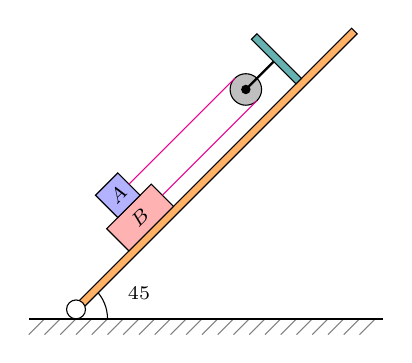
\begin{tikzpicture}[font=\scriptsize]
	\draw (.4,-.12) arc(0:45:.52);
	\begin{scope}[rotate=45]
		\draw[fill=orange!60] (0,-.05) rectangle(5,.05);
		\draw[fill=white] (0,0) circle(.12);
		\draw[fill=red!30] (1,.05) rectangle(1.8,.45)node[midway,rotate=45]{\(B\)};
        \draw[fill=blue!30] (1.2,.45) rectangle(1.6,.85)node[midway,rotate=45]{\(A\)};
		\draw[fill=gray!50] (3.5,.45) circle(.2);
        \draw[magenta] (1.8,.25)--(3.5,.25) (1.6,.65)--(3.5,.65);
		\draw[thick] (3.5,.45)--(4,.45);
		\fill (3.5,.45) circle(.06);
		\draw[fill=teal!60] (4,.05) rectangle(4.1,.85);
	\end{scope}
    \foreach \x in {-.6,-.4,...,3.8}
	    \draw[gray] (\x,-.32)--++(.2,.2);
    \draw[thick] (-.6,-.12)--(3.9,-.12);
    \node at(.8,0.2){ \qty{45}{\degree}};
\end{tikzpicture}
\begin{choices}
	\item\(\frac{1}{3}\)
	\item\(\frac{1}{4}\)
	\item\(\frac{1}{5}\)
	\item\(\frac{1}{6}\)
\end{choices}
\begin{answer}
    C\qquad 提示：极限法，假设木板竖直，则\(B\)向下运动，\(A\)向上运动。当刚好滑动时，\(A\)、\(B\)之间的摩擦力\(f_B\)与\(B\)木板之间的摩擦力\(f_{\max}\)都达到最大静摩擦力，对\(A\)和\(AB\)整体的受力分析如下图所示，\(T = \frac{\sqrt{2}}{2}mg + f_B\)，\(2T + f_{\max} = \frac{\sqrt{2}}{2}\cdot 3mg \)

\begin{tikzpicture}[>=stealth,font=\scriptsize]
    \coordinate (o) at(0,0);
    \draw[->] (o)--++(0,-1)node[below]{\(mg\)};
	\draw[->,magenta] (o)--++(45:1.5)node[right]{\(T\)};
	\draw[->,teal] (o)--++(45:-.8)node[left]{\(f_{B}\)};
	\draw[->,orange] (o)--++(135:1.2)node[above]{\(N_B\)};

	\coordinate (a) at(4,0);
	\draw[->] (a)--++(0,-2)node[below]{\(3mg\)};
	\draw[->,magenta] (a)--++(45:2)node[right]{\(2T\)};
	\draw[->,teal] (a)--++(45:1)node[below right]{\(f_{\max}\)};
	\draw[->,orange] (a)--++(135:1.5)node[above]{\(N\)};
\end{tikzpicture}
\end{answer}